\documentclass[11pt,spanish]{article}

% =========================================================
% PLANTILLA BASE PARA TAREAS ACADÉMICAS / INFORMES TÉCNICOS
% =========================================================

% --- Idioma y codificación para Tectonic / XeLaTeX ---
\usepackage[spanish,es-tabla]{babel}
\usepackage{fontspec}

% --- Márgenes / papel ---
\usepackage{geometry}
\geometry{a4paper, margin=2.7cm}

% --- Matemáticas ---
\usepackage{amsmath}

% --- Tablas, enlaces y elementos visuales ---
\usepackage{array}
\usepackage{tabularx}
\usepackage{booktabs}
\usepackage{longtable}
\usepackage{graphicx}
\usepackage{float}
\usepackage{xcolor}
\usepackage{tikz}
\usetikzlibrary{positioning,shapes.geometric,arrows.meta,calc}
\usepackage{enumitem}
\usepackage{ragged2e}
\usepackage{caption}
\captionsetup{skip=6pt}
\captionsetup[table]{position=top}
\captionsetup[figure]{position=bottom}
\usepackage{xurl}
\usepackage[hidelinks]{hyperref}

% --- Configuración de párrafo en bloque para evitar cortes en cajas de código ---
\makeatletter
\renewcommand\paragraph{\@startsection{paragraph}{4}{\z@}%
  {2.2ex \@plus1ex \@minus.2ex}%
  {0.8ex}%
  {\normalfont\normalsize\bfseries}}
\makeatother

% --- Listados de código con formato elegante ---
\usepackage{listings}

\definecolor{codebg}{rgb}{0.97,0.97,0.98}
\definecolor{codeframe}{rgb}{0.85,0.85,0.88}
\definecolor{commentgreen}{rgb}{0.13,0.54,0.13}
\definecolor{keywordblue}{rgb}{0.0,0.2,0.7}
\definecolor{stringpurple}{rgb}{0.6,0.1,0.4}

% --- Colores para esquemas y diagramas TikZ ---
\definecolor{softblue}{rgb}{0.88, 0.93, 1.0}
\definecolor{softgreen}{rgb}{0.88, 0.96, 0.88}
\definecolor{softorange}{rgb}{1.0, 0.92, 0.82}
\definecolor{softpurple}{rgb}{0.93, 0.88, 0.98}
\definecolor{softteal}{rgb}{0.85, 0.95, 0.95}
\definecolor{softyellow}{rgb}{1.0, 0.95, 0.80}

\lstdefinestyle{customcode}{
    backgroundcolor=\color{codebg},
    basicstyle=\ttfamily\footnotesize,
    breakatwhitespace=false,
    breaklines=true,
    captionpos=b,
    keepspaces=true,
    numbers=none,
    showspaces=false,
    showstringspaces=false,
    showtabs=false,
    tabsize=4,
    frame=single,
    rulecolor=\color{codeframe},
    commentstyle=\color{commentgreen}\itshape,
    keywordstyle=\color{keywordblue}\bfseries,
    stringstyle=\color{stringpurple},
    xleftmargin=0.5em,
    xrightmargin=0.5em
}

\lstdefinestyle{customcodenum}{
    backgroundcolor=\color{codebg},
    basicstyle=\ttfamily\footnotesize,
    breakatwhitespace=false,
    breaklines=true,
    captionpos=b,
    keepspaces=true,
    numbers=left,
    numbersep=6pt,
    numberstyle=\tiny\color{gray},
    showspaces=false,
    showstringspaces=false,
    showtabs=false,
    tabsize=4,
    frame=single,
    rulecolor=\color{codeframe},
    commentstyle=\color{commentgreen}\itshape,
    keywordstyle=\color{keywordblue}\bfseries,
    stringstyle=\color{stringpurple},
    xleftmargin=1.5em,
    xrightmargin=0.5em
}

\lstset{style=customcode}

% --- Encabezado y pie de página ---
\usepackage[myheadings]{fancyhdr}
\usepackage{lastpage}
\setlength{\headheight}{30pt}
\setlength{\footskip}{30pt}

% --- Interlineado ---
\linespread{1.2}
\sloppy

% =========================================================
% DATOS DEL DOCUMENTO
% =========================================================
\newcommand{\Institucion}{Instituto Tecnológico de Costa Rica}
\newcommand{\Campus}{Escuela de Ingeniería en Computación}
\newcommand{\DocumentoTitulo}{Progra00}
\newcommand{\DocumentoSubtitulo}{Arañador}
\newcommand{\NombreBuscador}{Encuadre}
\newcommand{\Curso}{IC-8060 Recuperación de Información Textual}
\newcommand{\Profesor}{Aurelio Sanabria}
\newcommand{\FechaDocumento}{1 de octubre de 2026}
\newcommand{\PeriodoAcademico}{II Semestre}
\newcommand{\AnioDocumento}{2026}

% Autores con nombre a la izquierda y carné a la derecha
\newcommand{\AutoresPortada}{%
\begin{minipage}{0.85\textwidth}
\begin{tabular*}{\linewidth}{@{\extracolsep{\fill}}lr@{}}
Santiago Espinoza Rendon & 2024156530 \\
Fabián Araya Ortega & 2019159110 \\
Mauricio González Prendas & 2024143009 \\
\end{tabular*}
\end{minipage}%
}

% Datos que aparecen en el encabezado
\newcommand{\DocHeaderLeft}{\Curso}
\newcommand{\DocHeaderRight}{\DocumentoTitulo}
\newcommand{\DocFooterRight}{Página~\thepage\ de~\pageref{LastPage}}

% Metadatos PDF
\title{\DocumentoTitulo}
\author{Santiago Espinoza Rendon, Fabián Araya Ortega, Mauricio González Prendas}
\date{\FechaDocumento}

% =========================================================
% CONFIGURACIÓN DE TABLAS Y UTILIDADES
% =========================================================
\newcolumntype{Y}{>{\RaggedRight\arraybackslash}X}
\newcolumntype{P}[1]{>{\RaggedRight\arraybackslash}p{#1}}
\renewcommand{\arraystretch}{1.22}
\setlength{\LTpre}{0.5em}
\setlength{\LTpost}{0.5em}

% =========================================================
% ENCABEZADO Y PIE
% =========================================================
\pagestyle{fancy}
\fancyhf{}
\fancyhead[L]{\DocHeaderLeft}
\fancyhead[R]{\DocHeaderRight}
\renewcommand{\headrulewidth}{0.4pt}
\renewcommand{\footrulewidth}{0.4pt}
\fancyfoot[R]{\DocFooterRight}

\fancypagestyle{widefancy}{%
    \fancyhf{}%
    \fancyhead[L]{\DocHeaderLeft}%
    \fancyhead[R]{\DocHeaderRight}%
    \renewcommand{\headrulewidth}{0.4pt}%
    \renewcommand{\footrulewidth}{0.4pt}%
    \fancyfoot[R]{\DocFooterRight}%
}

% =========================================================
% PORTADA
% =========================================================
\newcommand{\MakeCover}{%
\begin{titlepage}
\thispagestyle{empty}
\centering

{\bfseries \huge \Institucion \par}
\vspace{0.25cm}
{\LARGE \Campus \par}
\vspace{0.15cm}
{\LARGE \Curso \par}
\vspace{0.5cm}

\includegraphics[width=0.22\linewidth]{imgs/logo.png}

\vfill

{\huge \bfseries \DocumentoTitulo: \DocumentoSubtitulo \par}
\vspace{0.4cm}
{\Large \textit{\NombreBuscador} \par}

\vfill

{\bfseries \LARGE Profesor: \par}
\vspace{0.2cm}
{\Large \Profesor \par}

\vfill

{\bfseries \LARGE Estudiantes: \par}
\vspace{0.3cm}
{\Large \AutoresPortada \par}

\vfill

{\bfseries\LARGE Fecha: \par}
\vspace{0.2cm}
{\Large \FechaDocumento \par}

\vfill

{\LARGE \PeriodoAcademico \par}
{\LARGE \AnioDocumento \par}

\end{titlepage}%
}

% =========================================================
% DOCUMENTO
% =========================================================
\begin{document}
\hypersetup{pageanchor=false}

% =========================
% Portada
% =========================
\MakeCover

% =========================
% Índice
% =========================
\pagenumbering{roman}
\pagestyle{empty}
\tableofcontents
\clearpage
\pagenumbering{arabic}
\hypersetup{pageanchor=true}
\pagestyle{fancy}

% =========================================================
% CONTENIDO — PROGRA00: ARAÑADOR
% =========================================================

\section{Introducción}

\textit{\NombreBuscador} es un buscador enfocado en contenido audiovisual, es decir, cine, series, anime y guionismo. Los buscadores generales no responden bien preguntas como en qué película se dice exactamente tal frase o qué obras usan cierto recurso narrativo, por lo que el trabajo consistió en armar la parte de abajo del sistema, que es el arañador que baja las páginas junto con el repositorio de texto plano que queda listo para indexar después.

Para la misma necesidad de información se hicieron \textbf{dos arañadores que comparten semillas, políticas y almacenamiento}: uno propio, escrito en Python usando solo la biblioteca estándar, con hilos y descarga concurrente, y otro con bibliotecas existentes, Scrapy y Trafilatura. Los dos leen las mismas semillas de \texttt{Progra00/semillas.txt}, aplican las mismas políticas con los mismos valores, salvo el retardo base y la forma de extraer el texto, tal como se indica en cada política, y guardan los datos con el mismo esquema en SQLite sobre el almacenamiento único de \texttt{Progra00/almacenamiento/}, para que compararlos sea justo y para poder correr primero una implementación y luego la otra sin volver a descargar lo que ya está guardado.

\section{Necesidad de información}

\subsection{Tema central}

El tema es el \textbf{dominio audiovisual}, que abarca producciones cinematográficas, series de televisión, anime y todo lo que rodea al guion, como libretos, transcripciones, tropos narrativos, reseñas críticas y fichas técnicas. Lo escogimos porque en internet hay muchísimo texto público sobre esto, pero está regado en sitios muy distintos y los buscadores generales no son buenos para búsquedas como ``en qué película dicen exactamente tal frase'' o ``qué películas usan tal recurso narrativo'', mientras que un repositorio especializado con texto limpio sí puede responder ese tipo de preguntas.

\subsection{Características de la información que se descarga}

\begin{itemize}[label=\textbullet, leftmargin=*]
    \item \textbf{Tipo de contenido:} texto largo y con bastante densidad semántica, como guiones completos, transcripciones escena por escena, enciclopedias de tropos, reseñas y ensayos críticos, y fichas técnicas de películas, series y anime.
    \item \textbf{Idioma:} mixto, pues los sitios de guiones, tropos y crítica que usamos son mayormente en inglés, y Wikipedia en español y FilmAffinity aportan contenido en español. Es decir, el corpus es bilingüe con predominio del inglés, y eso lo tomamos en cuenta al analizar las estadísticas.
    \item \textbf{Formato final:} un archivo .txt en UTF-8 por página, ya sin HTML, scripts, estilos, menús ni anuncios.
    \item \textbf{Lo que no se descarga:} imágenes, audio, video, PDFs, comprimidos, ejecutables, hojas de estilo y JavaScript. La necesidad es de texto, así que todo lo demás solo gasta ancho de banda y disco.
    \item \textbf{Frescura:} los guiones casi no cambian, pero las fichas, reseñas y enciclopedias sí se corrigen o crecen con el tiempo, así que se revisitan cada 30 días.
\end{itemize}

\subsection{Tipo de consultas esperadas}

\begin{center}
\begin{tabularx}{\linewidth}{YYY}
\toprule
\textbf{Tipo de consulta} & \textbf{Qué busca la persona} & \textbf{Ejemplo} \\
\midrule
Diálogo exacto & Una línea o un intercambio entre personajes & ``Transcripción del diálogo de apertura de Pulp Fiction'' \\
Temática & Recursos narrativos y tropos & ``Uso del tropo del antihéroe en películas de ciencia ficción'' \\
Cruzada & Director, género o época combinados & ``Estilo de diálogo de Quentin Tarantino'' o ``temas comunes en el anime de ciencia ficción de los noventa'' \\
Por obra y escena & Un fragmento puntual de un guion & ``Guion completo de Interstellar escena del agujero negro'' \\
\bottomrule
\end{tabularx}
\end{center}

\subsection{Caracterización del colectivo}

\begin{center}
\begin{tabularx}{\linewidth}{lY}
\toprule
\textbf{Aspecto} & \textbf{Descripción} \\
\midrule
Quiénes son & Estudiantes de comunicación y cine, cineastas en formación, guionistas, gente que investiga narrativa audiovisual y aficionados al análisis crítico de medios. \\
Rango etario & De 18 a 45 años. \\
Contexto socioeconómico & Comunidad universitaria y técnica de Costa Rica y de la región hispanohablante, con computadora e internet, que quiere herramientas de búsqueda sin suscripciones ni pagos. \\
Subtemas de interés & Guiones de producción, análisis de tropos narrativos, narrativa comparada en animación y conservación digital de libretos. \\
Consultas esperadas & ``Guion completo de Interstellar escena del agujero negro''. ``Uso del tropo del antihéroe en películas de ciencia ficción''. ``Transcripción del diálogo de apertura de Pulp Fiction''. ``Evolución de tropos narrativos en series de anime clásicas''. \\
\bottomrule
\end{tabularx}
\end{center}

Como el colectivo es hispanohablante pero gran parte de los guiones están en inglés, asumimos que muchas personas van a hacer consultas mezcladas, por ejemplo con el título en inglés y la descripción en español. Por eso dejamos las dos lenguas en el corpus y no filtramos por idioma al descargar.

\section{Políticas de arañado}

\subsection{Arquitectura general}

Antes de las políticas conviene ver cómo funciona el sistema completo, pues las políticas se aplican en distintos puntos de este flujo y en cada una indicamos en cuál.

\begin{itemize}[label=\textbullet, leftmargin=*]
    \item \textbf{Inicialización:} se leen las 15 semillas de \texttt{Progra00/semillas.txt}, y los dominios permitidos se sacan de ahí mismo, pues no están escritos en el código.
    \item \textbf{Calendarización y descarga:} el calendarizador despacha las solicitudes respetando \texttt{robots.txt} y los retardos, y el motor de descarga hace las peticiones HTTP.
    \item \textbf{Bitácora:} cada respuesta o error se registra en la tabla \texttt{bitacora\_recorrido} con dominio, código HTTP y tiempo de respuesta.
    \item \textbf{Extracción:} se saca el texto principal de la página, quitando menús, scripts y anuncios.
    \item \textbf{Validación:} se descarta lo que sea muy corto o con poca proporción de letras y números, y se calculan los hashes SHA-256 de la URL y del contenido.
    \item \textbf{Persistencia:} se revisa si hay duplicados, se escribe el .txt de forma atómica mediante archivo temporal, fsync y renombrado, y se insertan los metadatos en SQLite.
    \item \textbf{Frescura:} si un documento ya guardado cumplió su fecha de revisita, se vuelve a bajar y se actualiza, sin crear archivos repetidos.
\end{itemize}

\begin{figure}[H]
\centering
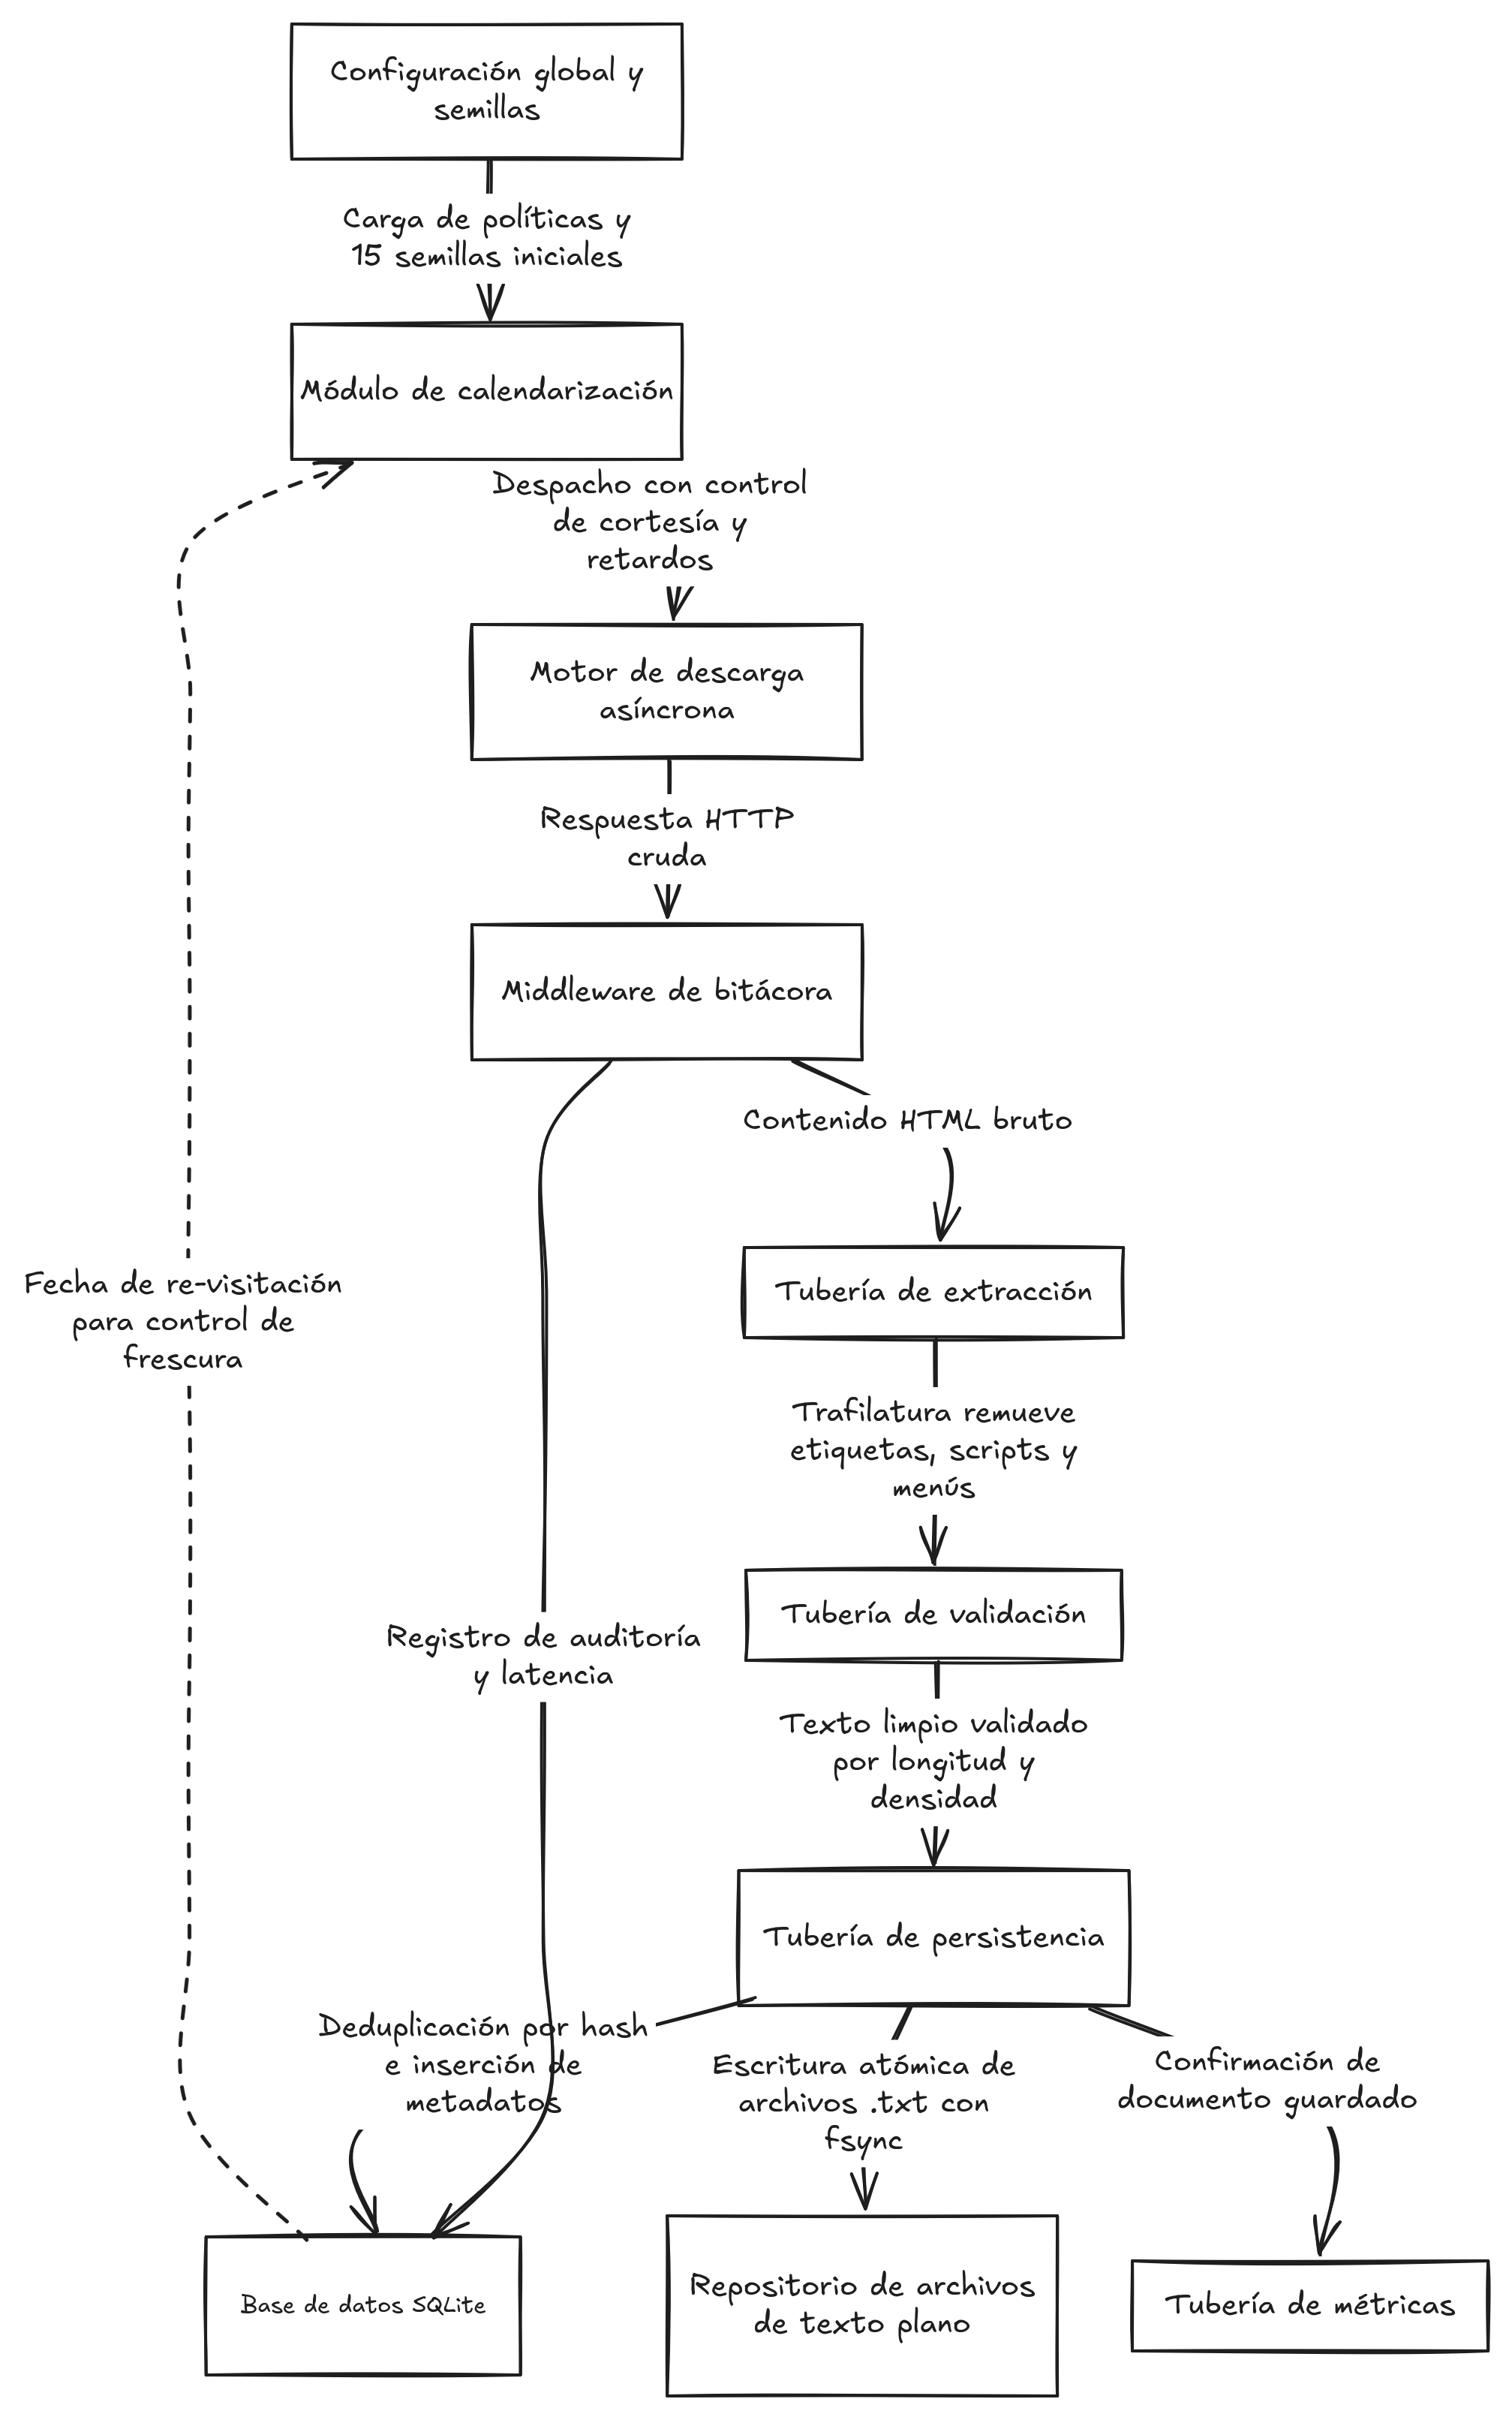
\includegraphics[width=0.85\linewidth]{imgs/diagrama01.png}
\caption{Arquitectura general del sistema de arañado.}
\label{fig:arquitectura}
\end{figure}

\subsection{Metadatos que hay que almacenar}

Varias políticas necesitan ``memoria'' para funcionar, pues, por ejemplo, no se puede saber si un documento está vencido sin guardar cuándo se descargó. Estos son los campos que guardamos en SQLite y para qué política sirve cada uno.

\textbf{Tabla \texttt{documentos}, con una fila por documento guardado:}

\begin{center}
\begin{tabularx}{\linewidth}{lYY}
\toprule
\textbf{Campo} & \textbf{Para qué sirve} & \textbf{Políticas} \\
\midrule
\texttt{url, hash\_url} & URL canónica y su huella SHA-256, ambas únicas & P12 deduplicación, P13 frescura \\
\texttt{hash\_contenido} & Huella SHA-256 del texto limpio, que también es el nombre del archivo & P12 deduplicación \\
\texttt{dominio, categoria} & Sitio de origen y categoría, por ahora siempre con valor documentos, y definen la carpeta donde queda el archivo, con la forma \path{dominio/documentos/xx/hash.txt} & P1 hosts, estadísticas por dominio \\
\texttt{ruta\_relativa} & Dónde está el .txt dentro del repositorio & Consistencia archivo/base de datos \\
\texttt{tamano\_texto\_bytes} & Tamaño del texto guardado & P5 calidad, meta de 10 GB \\
\texttt{codigo\_http} & Código con que respondió el servidor & P15 auditoría \\
\texttt{profundidad} & Saltos de enlace desde la semilla & P2 profundidad, P6 amplitud \\
\texttt{fecha\_descarga, fecha\_revisitacion} & Cuándo se bajó y cuándo toca volver a revisarlo & P13 frescura \\
\bottomrule
\end{tabularx}
\end{center}

\textbf{Tabla \texttt{bitacora\_recorrido}, con una fila por intento de descarga:}

\begin{center}
\begin{tabularx}{\linewidth}{lY}
\toprule
\textbf{Campo} & \textbf{Para qué sirve} \\
\midrule
\texttt{timestamp} & Momento del intento \\
\texttt{dominio} & Sitio consultado, lo que demuestra que el recorrido no se quedó en un solo sitio \\
\texttt{url\_origen, url\_destino} & De qué página salió el enlace y a cuál se fue, o sea el camino de la araña \\
\texttt{tiempo\_respuesta\_ms} & Latencia observada y base para ajustar el retardo según P10 \\
\texttt{codigo\_http} & Resultado de la petición \\
\texttt{accion} & Qué pasó: respuesta, error, baja densidad, duplicado, almacenado, revisitado y, solo en la versión propia, bloqueado por robots, noindex o no HTML \\
\bottomrule
\end{tabularx}
\end{center}

Además guardamos por host las reglas de \texttt{robots.txt}, en memoria durante la ejecución, y, para poder reanudar, la frontera de URLs pendientes, que es una tabla compartida \texttt{frontera} en la misma base SQLite, con una fila por URL cuya clave es el SHA-256 de la URL, o sea \texttt{hash\_url}, donde se guardan la URL, su profundidad, la prioridad, que es el negativo de la profundidad para el recorrido en amplitud, la URL de origen, el estado, ya sea \texttt{pendiente}, \texttt{visitada} o \texttt{error}, los intentos y la fecha de actualización. Las dos implementaciones leen y escriben esa misma tabla, así que la cola sobrevive al cambio de una a otra.

\subsection{Las políticas}

Cada política tiene nombre, descripción, justificación con referencia a la necesidad de información y al colectivo, metadatos y el lugar donde se implementa en cada arañador. El código de cada archivo lo listamos sin números de línea, porque cambian con cualquier edición.

\subsubsection{Políticas de selección}

Estas políticas definen qué contenido se descarga.

\paragraph{P1. Hosts permitidos}

\begin{itemize}[label=\textbullet, leftmargin=*]
    \item \textbf{Descripción:} la araña solo sigue enlaces de los dominios de las semillas o sus subdominios. Ningún dominio está escrito en el código, pues se derivan de \texttt{Progra00/semillas.txt}. Con las 15 semillas actuales quedan 10 dominios.
    \item \textbf{Justificación:} sin este límite, la araña saldría del tema a los pocos saltos hacia redes sociales, tiendas o publicidad, pues el colectivo quiere contenido audiovisual y no navegar por la web entera, lo que corresponde a la política de ``recorrido enfocado'' que describen Manning et al.\ (2008, cap.\ 20).
    \item \textbf{Metadatos:} dominio.
    \item \textbf{Dónde:}
    \begin{itemize}[label=--, leftmargin=*]
        \item Scrapy: \texttt{arana\_semillas.py}.
        \item Propia: \texttt{semillas.host\_permitido} y \texttt{Arana.url\_aceptable}.
    \end{itemize}
\end{itemize}

\paragraph{P2. Límite de profundidad}

\begin{itemize}[label=\textbullet, leftmargin=*]
    \item \textbf{Descripción:} máximo 4 saltos de enlace desde una semilla, y al llegar al límite no se agregan más enlaces.
    \item \textbf{Justificación:} los sitios tienen trampas de rastreo, como calendarios, filtros y parámetros que generan URLs infinitas, y cuanto más lejos de la semilla, más probable es caer en secciones administrativas que no sirven para el colectivo, como describen Olston y Najork (2010) al tratar estas trampas como uno de los problemas clásicos de los arañadores.
    \item \textbf{Metadatos:} profundidad.
    \item \textbf{Dónde:}
    \begin{itemize}[label=--, leftmargin=*]
        \item Scrapy: \texttt{DEPTH\_LIMIT = 4} en \texttt{configuracion.py} y \texttt{arana\_semillas.py}.
        \item Propia: \texttt{Arana.encolar} y \texttt{Arana.\_procesar}.
    \end{itemize}
\end{itemize}

\paragraph{P3. Exclusión de formatos binarios}

\begin{itemize}[label=\textbullet, leftmargin=*]
    \item \textbf{Descripción:} se descartan 49 extensiones de imágenes, audio, video, PDFs, comprimidos, ejecutables, CSS, JS y demás, tanto en la configuración de Scrapy como en la versión propia. La tubería de validación de Scrapy trae además su propia lista de respaldo, un poco más corta, por si alguna araña enlaza un tipo indebido, mientras que la versión propia solo procesa respuestas cuyo Content-Type sea HTML y la de Scrapy solo procesa respuestas de texto.
    \item \textbf{Justificación:} el repositorio pedido es de texto plano, por lo que bajar audio o video llenaría el disco y el ancho de banda con cosas que el colectivo no puede buscar como texto. Se filtra dos veces, tanto por extensión en la URL como por tipo de contenido, porque hay URLs sin extensión que devuelven binarios.
    \item \textbf{Metadatos:} extensión de la ruta y Content-Type, evaluados al vuelo sin guardarlos.
    \item \textbf{Dónde:}
    \begin{itemize}[label=--, leftmargin=*]
        \item Scrapy: \texttt{EXTENSIONES\_EXCLUIDAS} en \texttt{configuracion.py}, \texttt{arana\_semillas.py} y \texttt{tuberia\_validacion.py}.
        \item Propia: \texttt{Arana.url\_aceptable} y \texttt{Respuesta.es\_html}.
    \end{itemize}
\end{itemize}

\paragraph{P4. Tamaño máximo de respuesta y largo de URL}

\begin{itemize}[label=\textbullet, leftmargin=*]
    \item \textbf{Descripción:} se ignoran respuestas de más de 5 MB y URLs de más de 2048 caracteres.
    \item \textbf{Justificación:} una página HTML normal con guion o reseña pesa mucho menos de 5 MB, y lo que pasa de ahí casi siempre es un archivo mal etiquetado. Las URLs larguísimas suelen ser parámetros de rastreo o trampas (Olston y Najork, 2010), por lo que así se protege la memoria sin perder contenido útil para el colectivo.
    \item \textbf{Metadatos:} ninguno adicional, pues se evalúa sobre la respuesta.
    \item \textbf{Dónde:}
    \begin{itemize}[label=--, leftmargin=*]
        \item Scrapy: \texttt{DOWNLOAD\_MAXSIZE} y \texttt{URLLENGTH\_LIMIT}.
        \item Propia: \texttt{Descargador.\_descargar\_con\_turno} y \texttt{Arana.url\_aceptable}.
    \end{itemize}
\end{itemize}

\paragraph{P5. Calidad y densidad textual}

\begin{itemize}[label=\textbullet, leftmargin=*]
    \item \textbf{Descripción:} después de extraer el texto principal, se exige un mínimo de 300 caracteres y al menos 35 \% de caracteres alfanuméricos, y si no cumple, se descarta y se anota en la bitácora.
    \item \textbf{Justificación:} lo que el colectivo busca son guiones, ensayos y fichas, o sea prosa, mientras que las páginas de error, los índices de enlaces y los ``cascarones'' vacíos ensucian el repositorio y las estadísticas, por ejemplo la curva de Zipf. La extracción de contenido principal descartando la ``plantilla'' de la página es un problema conocido, que Barbaresi (2021) trata en Trafilatura, la biblioteca que usa la versión con Scrapy.
    \item \textbf{Metadatos:} \texttt{tamano\_texto\_bytes} y la acción \texttt{BAJA\_DENSIDAD} en la bitácora.
    \item \textbf{Dónde:}
    \begin{itemize}[label=--, leftmargin=*]
        \item Scrapy: \texttt{tuberia\_extraccion.py} y \texttt{tuberia\_validacion.py}.
        \item Propia: \texttt{extraccion.motivo\_rechazo}.
    \end{itemize}
\end{itemize}

\paragraph{P6. Recorrido en amplitud}

\begin{itemize}[label=\textbullet, leftmargin=*]
    \item \textbf{Descripción:} las URLs de menor profundidad se procesan primero, así que la araña explora por capas y no se mete de lleno en un solo sitio.
    \item \textbf{Justificación:} queremos cobertura amplia de obras y géneros antes de profundizar en un catálogo específico, lo que además ayuda a que el recorrido sea diverso, como pide la bitácora, y Cho, García-Molina y Page (1998) y Najork y Wiener (2001) muestran que el recorrido en amplitud tiende a encontrar primero las páginas de mejor calidad.
    \item \textbf{Metadatos:} profundidad, además de la prioridad de la solicitud, guardada en memoria.
    \item \textbf{Dónde:}
    \begin{itemize}[label=--, leftmargin=*]
        \item Scrapy: \texttt{filtro\_duplicados.py}, que resta prioridad según la profundidad.
        \item Propia: \texttt{Arana.frontera}, una PriorityQueue ordenada por profundidad.
    \end{itemize}
\end{itemize}

\subsubsection{Políticas de cortesía}

Estas políticas definen cómo se descarga.

\paragraph{P7. Respeto a robots.txt}

\begin{itemize}[label=\textbullet, leftmargin=*]
    \item \textbf{Descripción:} antes de pedir cualquier URL se consulta el \texttt{robots.txt} de su servidor y no se descarga lo que esté prohibido, y la versión propia además respeta Crawl-delay.
    \item \textbf{Justificación:} es la norma ética básica de los arañadores y el estándar formal del Protocolo de Exclusión de Robots (Koster, 1994; IETF RFC 9309, 2022), y como muchos de los sitios son comunitarios o de aficionados, no queremos que nos bloqueen ni causar problemas.
    \item \textbf{Metadatos:} reglas de \texttt{robots.txt} por host, en memoria, y la versión propia además anota la acción \texttt{BLOQUEADO\_ROBOTS} en la bitácora, mientras que en Scrapy el bloqueo lo hace su propio módulo de \texttt{robots.txt} y no queda con acción propia.
    \item \textbf{Dónde:}
    \begin{itemize}[label=--, leftmargin=*]
        \item Scrapy: \texttt{ROBOTSTXT\_OBEY = True}.
        \item Propia: \texttt{Descargador.permitido\_por\_robots}.
    \end{itemize}
\end{itemize}

\paragraph{P8. Identificación del robot}

\begin{itemize}[label=\textbullet, leftmargin=*]
    \item \textbf{Descripción:} cada petición lleva el mismo User-Agent descriptivo en las dos implementaciones, \texttt{AranadorAudiovisualBot/1.0}, con un enlace institucional del curso.
    \item \textbf{Justificación:} permite que los administradores de los sitios distingan una araña académica de un ataque y, si hay algún problema, sepan quién es, sin poner ningún correo personal, y el estándar de \texttt{robots.txt} usa justamente el nombre del agente para aplicar reglas según el RFC 9309, así que identificarse bien también sirve para que las reglas de cada sitio se apliquen correctamente.
    \item \textbf{Metadatos:} encabezado User-Agent, configurable en \texttt{.env}.
    \item \textbf{Dónde:}
    \begin{itemize}[label=--, leftmargin=*]
        \item Scrapy: \texttt{USER\_AGENT} en \texttt{configuracion.py}.
        \item Propia: \texttt{configuracion.USER\_AGENT}.
    \end{itemize}
\end{itemize}

\paragraph{P9. Cortesía a nivel de documento con noindex y nofollow}

\begin{itemize}[label=\textbullet, leftmargin=*]
    \item \textbf{Descripción:} se leen la etiqueta \path{<meta name="robots">} y el encabezado \texttt{X-Robots-Tag}, de modo que con \texttt{noindex} no se guarda el texto de esa página, con \texttt{nofollow} no se siguen sus enlaces y \texttt{none} aplica ambos.
    \item \textbf{Justificación:} \texttt{robots.txt} controla el acceso por ruta, pero cada autor puede pedir que una página puntual no se indexe, por lo que respetarlo es coherente con la política P7 y con lo que dice la documentación de los buscadores sobre estas directivas.
    \item \textbf{Metadatos:} directivas de la página, evaluadas al vuelo, y la versión propia anota la acción \texttt{NOINDEX} en la bitácora, mientras que en Scrapy la página simplemente no se emite como documento.
    \item \textbf{Dónde:}
    \begin{itemize}[label=--, leftmargin=*]
        \item Scrapy: \texttt{arana\_semillas.py}.
        \item Propia: \texttt{extraccion.\_Analizador} y \texttt{Arana.\_procesar}, pasos 5 y 6.
    \end{itemize}
\end{itemize}

\paragraph{P10. Retardo y concurrencia por dominio}

\begin{itemize}[label=\textbullet, leftmargin=*]
    \item \textbf{Descripción:} nunca más de 4 descargas simultáneas al mismo dominio, con un retardo base entre solicitudes de 0,5 s en Scrapy y 0,75 s en la versión propia, que se adapta a la latencia del servidor hasta un máximo de 5 s, donde en Scrapy lo hace AutoThrottle, mientras que en la propia, además, la pausa se duplica cuando el servidor responde con 429 o 5xx.
    \item \textbf{Justificación:} Manning et al.\ (2008, cap.\ 20) recomiendan espaciar las peticiones al mismo servidor para no saturarlo, y como los sitios de guiones y tropos son comunitarios, con poca infraestructura, un ritmo agresivo los tumbaría o nos haría bloquear.
    \item \textbf{Metadatos:} \texttt{tiempo\_respuesta\_ms} y \texttt{codigo\_http} en la bitácora, pues la latencia observada alimenta el ajuste.
    \item \textbf{Dónde:}
    \begin{itemize}[label=--, leftmargin=*]
        \item Scrapy: \texttt{DOWNLOAD\_DELAY}, \texttt{CONCURRENT\_REQUESTS\_PER\_DOMAIN} y \texttt{AUTOTHROTTLE\_*}.
        \item Propia: clase \texttt{ControlCortesia} en \texttt{descargador.py}.
    \end{itemize}
\end{itemize}

\paragraph{P11. Reintentos con espera}

\begin{itemize}[label=\textbullet, leftmargin=*]
    \item \textbf{Descripción:} hasta 3 reintentos ante 429, 500, 502, 503, 504, 522 y 524 y ante errores de red, con timeout de 45 s. La versión propia espera 2, 4 y 8 s entre intentos, con espera exponencial, mientras que Scrapy usa su módulo de reintentos, que reintenta sin esa espera, aunque AutoThrottle modera el ritmo.
    \item \textbf{Justificación:} estos códigos suelen ser fallas temporales o el servidor pidiendo que bajemos el ritmo, por lo que reintentar sin espera puede empeorar el problema, pero no reintentar perdería documentos válidos que el colectivo podría necesitar. El código 429, de demasiadas solicitudes, está definido en el RFC 6585 y los 5xx en el RFC 9110.
    \item \textbf{Metadatos:} \texttt{codigo\_http} y acción \texttt{ERROR} en la bitácora.
    \item \textbf{Dónde:}
    \begin{itemize}[label=--, leftmargin=*]
        \item Scrapy: \texttt{RETRY\_*} en \texttt{configuracion.py}.
        \item Propia: \texttt{Descargador.descargar}.
    \end{itemize}
\end{itemize}

\subsubsection{Políticas de revisitación}

Estas políticas definen qué contenido se vuelve a bajar.

\paragraph{P12. Deduplicación por URL y por contenido}

\begin{itemize}[label=\textbullet, leftmargin=*]
    \item \textbf{Descripción:} se calcula el SHA-256 de la URL canónica, sin parámetros de rastreo ni fragmentos, y del texto limpio, de modo que una URL ya guardada y vigente no se baja otra vez, y si dos URLs distintas dan el mismo texto, se guarda un solo archivo.
    \item \textbf{Justificación:} el mismo guion aparece enlazado desde rutas espejo o con parámetros distintos, y guardarlo varias veces inflaría el repositorio, pues los 10 GB deben ser de contenido distinto, además de sesgar las estadísticas de palabras. La detección de duplicados la tratan Manning et al.\ (2008, cap.\ 19), mientras que nosotros hacemos duplicados exactos por hash. Los casi-duplicados (Broder et al., 1997) quedaron fuera del alcance.
    \item \textbf{Metadatos:} \texttt{hash\_url}, \texttt{hash\_contenido}.
    \item \textbf{Dónde:}
    \begin{itemize}[label=--, leftmargin=*]
        \item Scrapy: \texttt{tuberia\_almacenamiento.py} y \texttt{repositorio.py}.
        \item Propia: \texttt{Arana.encolar} y \texttt{BaseDatos.guardar\_documento}.
    \end{itemize}
\end{itemize}

\paragraph{P13. Control de frescura}

\begin{itemize}[label=\textbullet, leftmargin=*]
    \item \textbf{Descripción:} cada documento tiene una fecha de revisita a 30 días de su descarga, por lo que antes de 30 días no se vuelve a pedir, pero después sí, y si el contenido cambió se guarda la versión nueva y se borra el archivo anterior, para no dejar copias repetidas.
    \item \textbf{Justificación:} las fichas, reseñas y enciclopedias se corrigen y crecen, pero bajar todo otra vez cada día sería un desperdicio y una carga para los sitios, así que el colectivo encuentra fichas y reseñas actualizadas, en línea con el balance entre frescura y costo de las políticas de refresco que estudian Cho y García-Molina (2003).
    \item \textbf{Metadatos:} \texttt{fecha\_descarga}, \texttt{fecha\_revisitacion}.
    \item \textbf{Dónde:}
    \begin{itemize}[label=--, leftmargin=*]
        \item Scrapy: \texttt{filtro\_duplicados.py} y \texttt{repositorio.necesita\_revisita}.
        \item Propia: \texttt{BaseDatos.necesita\_revisita} y \texttt{guardar\_documento}.
    \end{itemize}
\end{itemize}

\subsubsection{Políticas de ejecución y auditoría}

\paragraph{P14. Descarga concurrente}

\begin{itemize}[label=\textbullet, leftmargin=*]
    \item \textbf{Descripción:} la versión propia usa 16 hilos trabajadores que descargan al mismo tiempo, y si un host ya está lleno, el hilo devuelve la URL a la cola y toma otra de un host libre, mientras que Scrapy usa su motor asíncrono.
    \item \textbf{Justificación:} para llegar a 10 GB hay que descargar en paralelo, porque la mayor parte del tiempo se va esperando la red, pero el paralelismo se reparte entre dominios para no chocar con P10, pues los arañadores de escala real son multihilo o asíncronos por la misma razón (Heydon y Najork, 1999).
    \item \textbf{Metadatos:} ninguno adicional.
    \item \textbf{Dónde:}
    \begin{itemize}[label=--, leftmargin=*]
        \item Scrapy: reactor de Twisted y \texttt{CONCURRENT\_REQUESTS}.
        \item Propia: \texttt{Arana.\_trabajador} y \texttt{Arana.ejecutar}.
    \end{itemize}
\end{itemize}

\paragraph{P15. Auditoría del recorrido con bitácora}

\begin{itemize}[label=\textbullet, leftmargin=*]
    \item \textbf{Descripción:} cada intento queda registrado en SQLite y en un log de texto, ya sea respuesta, error, bloqueo, descarte o guardado.
    \item \textbf{Justificación:} el enunciado pide demostrar que la araña no bajó todo de un solo sitio, y con la bitácora se puede consultar cuántas visitas hubo por dominio, con qué latencia y qué se descartó y por qué. En Scrapy las acciones registradas son \texttt{RESPUESTA}, \texttt{ERROR}, \texttt{ALMACENADO}, \texttt{REVISITADO}, \texttt{DUPLICADO\_URL}, \texttt{DUPLICADO\_CONTENIDO} y \texttt{BAJA\_DENSIDAD}, mientras que la propia agrega \texttt{BLOQUEADO\_ROBOTS}, \texttt{NOINDEX} y \texttt{NO\_HTML}.
    \item \textbf{Metadatos:} todos los campos de \texttt{bitacora\_recorrido}.
    \item \textbf{Dónde:}
    \begin{itemize}[label=--, leftmargin=*]
        \item Scrapy: \texttt{intermediario\_bitacora.py} y \texttt{repositorio.py}.
        \item Propia: \texttt{Arana.\_procesar} y \texttt{cli.configurar\_log}, en el archivo \texttt{bitacoras/recorrido.log}.
    \end{itemize}
\end{itemize}

\section{Estadísticas del repositorio}

\subsection{Cómo se calcularon}

Las estadísticas se sacan con \texttt{uv run arañador informe}, un único comando que lee el almacenamiento compartido \texttt{Progra00/almacenamiento/}, o sea la base SQLite con los metadatos y el repositorio de texto plano, sin importar cuál de los dos arañadores hizo la descarga, y escribe en \texttt{Progra00/resultados/}, pues estas rutas derivan de \texttt{RAIZ\_DATOS}. El comando concilia los archivos en disco con la base de datos y da tamaño, cantidad de documentos y distribución por dominio, y además recorre todos los .txt, tokeniza en minúsculas en Unicode con acentos y cuenta frecuencias para la ley de Zipf. No existe un comando de informe en la versión propia, pues el resultado es el mismo sin importar qué implementación descargó.

\subsection{Distribución por dominio}

\begin{center}
\begin{tabularx}{\linewidth}{lYYY}
\toprule
\textbf{Dominio} & \textbf{Documentos} & \textbf{Tamaño, en GiB} & \textbf{\% de documentos} \\
\midrule
tvtropes.org & 159\,234 & 3,2435 & 36,45 \\
es.wikipedia.org & 119\,316 & 1,3411 & 27,31 \\
animenewsnetwork.com & 101\,473 & 0,5458 & 23,23 \\
tvmaze.com & 36\,316 & 0,0318 & 8,31 \\
sensesofcinema.com & 14\,427 & 0,2706 & 3,30 \\
simplyscripts.com & 3\,388 & 0,0674 & 0,78 \\
filmaffinity.com & 1\,947 & 0,0034 & 0,45 \\
dailyscript.com & 759 & 0,0961 & 0,17 \\
imsdb.com & 20 & 0,0022 & 0,005 \\
subslikescript.com & 0 & 0,0000 & 0,00 \\
\midrule
\textbf{Total} & \textbf{436\,880} & \textbf{5,6018} & \textbf{100,00} \\
\bottomrule
\end{tabularx}
\end{center}

subslikescript.com no aportó documentos porque sus páginas se descartaron por baja densidad tras la extracción, e imsdb.com aportó solo 20 por la misma razón, aunque es un dominio con muchos guiones, mientras que la mayor parte del corpus provino de tvtropes.org, es.wikipedia.org y animenewsnetwork.com.

\subsection{Frecuencia de palabras y ley de Zipf}

La ley de Zipf (Zipf, 1949) dice que la frecuencia de una palabra es aproximadamente inversamente proporcional a su posición en el ranking de frecuencias, lo que se expresa como $f(r) \approx C / r$. Al graficarlo en escala logarítmica en ambos ejes debería verse casi una línea recta con pendiente cercana a $-$1 (Manning et al., 2008, cap.\ 5). Es una buena prueba de sanidad del corpus, pues si la curva se parece a Zipf, el texto es lenguaje natural y no basura repetida.

\begin{figure}[H]
\centering
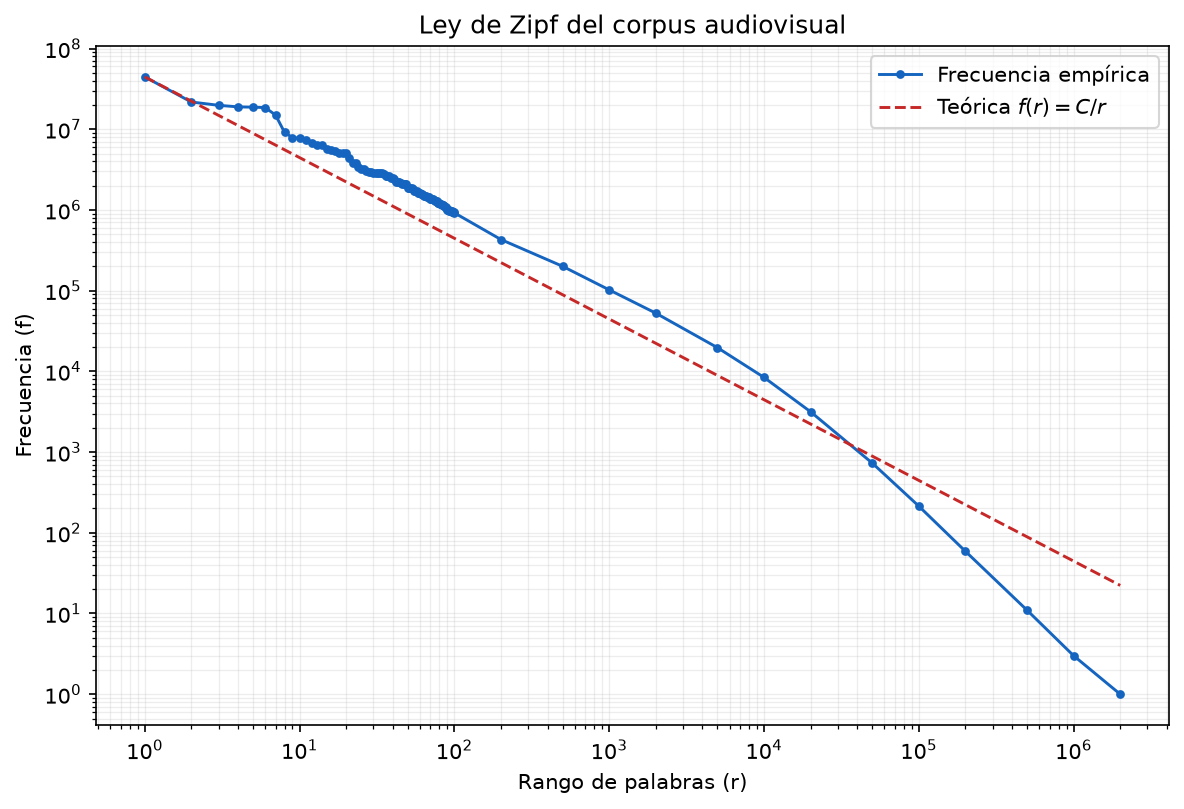
\includegraphics[width=0.8\linewidth]{imgs/grafica_ley_zipf.png}
\caption{Curva de Zipf del corpus, con la frecuencia empírica frente a la teórica $f(r)=C/r$ en escala logarítmica doble.}
\label{fig:zipf}
\end{figure}

La curva empírica de la figura~\ref{fig:zipf} sigue de cerca la recta teórica $f(r)=C/r$ en casi todo el rango, con la constante $C = 44\,572\,877$, que es la frecuencia de la palabra más común, «the», lo que confirma que el corpus es lenguaje natural y no texto repetido. La lista de palabras más frecuentes refleja que el material es bilingüe con predominio del inglés, pues a «the» le siguen «a», «to», «of», «and», «in», «is», «that», «with», «as», «for», «he» y «on», mezcladas con las voces españolas «de», «la», «el», «en», «y», «que» y «los», lo que es coherente con los sitios en inglés (tvtropes, imsdb, la crítica) y con la Wikipedia y FilmAffinity en español.

El vocabulario también delata el dominio audiovisual, pues aparecen términos propios de guion y crítica como «scene» con 268\,946 apariciones, «cut» con 166\,310, «act» con 159\,503, «int» con 76\,187, «ext» con 46\,409, «fade» con 15\,020, «voz» con 39\,000, «escena» con 25\,246 e «interior» con 37\,943. La cola es muy larga, pues 1\,313\,471 palabras, o sea el 45,9\% del vocabulario, aparecen una sola vez, sobre todo nombres propios, topónimos y variantes de escritura, que es exactamente lo que se espera en un corpus real.

\begin{center}
\small
\begin{tabular}{rrlr}
\toprule
\textbf{Rango} & \textbf{Frecuencia} & \textbf{Frecuencia relativa} & \textbf{Palabra} \\
\midrule
1 & 44\,572\,877 & 4,57\,\% & the \\
2 & 21\,765\,805 & 2,23\,\% & a \\
3 & 19\,798\,138 & 2,03\,\% & to \\
4 & 18\,942\,566 & 1,94\,\% & de \\
5 & 18\,767\,444 & 1,92\,\% & of \\
6 & 18\,558\,815 & 1,90\,\% & and \\
7 & 15\,008\,604 & 1,54\,\% & in \\
8 & 9\,166\,664 & 0,94\,\% & is \\
9 & 7\,870\,148 & 0,81\,\% & la \\
10 & 7\,775\,756 & 0,80\,\% & el \\
\bottomrule
\end{tabular}
\end{center}

\subsection{Comandos para reproducir}

\begin{lstlisting}
cd Progra00/arañador
uv run arañador informe
\end{lstlisting}

\section{URLs semilla}

Empezamos con 15 URLs, todas en \texttt{Progra00/semillas.txt}, que comparten las dos arañas. Pertenecen a 10 dominios y las escogimos para cubrir todos los tipos de información de la sección 2, como guiones, transcripciones, tropos, fichas, enciclopedia y crítica.

\begin{center}
\small
\begin{tabular}{c p{6.8cm} p{6.2cm}}
\toprule
\textbf{\#} & \textbf{URL} & \textbf{Tipo de contenido} \\
\midrule
1 & \url{https://imsdb.com/all-scripts.html} & Guiones de cine, índice general \\
2 & \url{https://www.dailyscript.com/movie.html} & Guiones de cine \\
3 & \url{https://www.simplyscripts.com/movie-scripts.html} & Guiones de cine \\
4 & \url{https://subslikescript.com/movies} & Transcripciones de películas \\
5 & \url{https://subslikescript.com/series} & Transcripciones de series \\
6 & \url{https://tvtropes.org/pmwiki/pmwiki.php/Main/Film} & Tropos en cine \\
7 & \url{https://tvtropes.org/pmwiki/pmwiki.php/Main/Anime} & Tropos en anime \\
8 & \url{https://www.filmaffinity.com/es/cat_new_th_es.html} & Fichas y reseñas en español \\
9 & \url{https://www.tvmaze.com/shows} & Fichas de series \\
10 & \url{https://www.animenewsnetwork.com/encyclopedia/} & Enciclopedia de anime \\
11 & \url{https://es.wikipedia.org/wiki/Portal:Cine} & Enciclopedia en español, cine \\
12 & \url{https://es.wikipedia.org/wiki/Categor%C3%ADa:Series_de_anime} & Enciclopedia en español, anime \\
13 & \url{https://www.sensesofcinema.com/} & Ensayos y crítica cinematográfica \\
14 & \url{https://es.wikipedia.org/wiki/Categor%C3%ADa:Pel%C3%ADculas_de_ciencia_ficci%C3%B3n} & Enciclopedia en español, ciencia ficción \\
15 & \url{https://tvtropes.org/pmwiki/pmwiki.php/Main/Plots} & Tropos y estructuras argumentales \\
\bottomrule
\end{tabular}
\end{center}

Sobre derechos de autor, muchos guiones y reseñas tienen derechos reservados. El corpus lo armamos solo con fines académicos para el curso, respetando \texttt{robots.txt} y sin redistribuirlo públicamente.

\section{Las dos implementaciones y su comparación}

\subsection{Arañador propio en Python con solo la biblioteca estándar}

No tiene dependencias externas, pues usa urllib para HTTP, \texttt{html.parser} para leer el HTML, \texttt{urllib.robotparser} para \texttt{robots.txt}, threading y queue para la concurrencia, y sqlite3 para los metadatos.

\begin{center}
\begin{tabularx}{\linewidth}{lY}
\toprule
\textbf{Archivo} & \textbf{Responsabilidad} \\
\midrule
\texttt{configuracion.py} & Lee .env y define los valores de todas las políticas \\
\texttt{semillas.py} & Lee las semillas y deriva los hosts permitidos \\
\texttt{descargador.py} & HTTP, robots.txt, cortesía por host y reintentos \\
\texttt{extraccion.py} & Texto limpio, enlaces y meta robots, además de la validación de calidad \\
\texttt{arana.py} & Frontera en amplitud, hilos trabajadores y guardado atómico \\
\texttt{bd.py} & SQLite con el mismo esquema que la versión con Scrapy \\
\texttt{cli.py} & Comando propio y bitácora en texto \\
\bottomrule
\end{tabularx}
\end{center}

El funcionamiento de un hilo consiste en sacar una URL de la frontera, revisar \texttt{robots.txt}, reservar un turno en su host, descargar, registrar en la bitácora, analizar el HTML, encolar los enlaces con profundidad + 1, salvo que haya nofollow, validar la calidad del texto, salvo que haya noindex, y por último calcular los hashes, escribir el .txt y guardar los metadatos, y la frontera se conserva en la tabla compartida \texttt{frontera}, por lo que al presionar Ctrl+C y volver a ejecutar se reanuda desde donde iba, y al arrancar, la araña reconcilia la tabla, descarta lo que ya está fresco en \texttt{documentos} y encola el resto.

\subsection{Arañador con las bibliotecas Scrapy y Trafilatura}

\textbf{¿Por qué Scrapy?} La razón principal es que preferimos usar Python en las dos implementaciones, y así evitamos reescribir las partes que son iguales en ambas: la lectura de semillas, la normalización de URLs, el cálculo de hashes, el esquema de SQLite, la estructura de carpetas del repositorio y los scripts de estadísticas y de Zipf. Con Nutch o crawler4j, que están escritos en Java, habríamos tenido que rehacer todo eso o armar puentes entre lenguajes, mientras que con las dos arañas en Python y con el mismo esquema, la comparación entre la solución propia y la de biblioteca es más justa, porque lo único que cambia es la herramienta de rastreo.

Usa \textbf{Scrapy} para el rastreo, \textbf{Trafilatura} para extraer el texto principal de cada página y SQLite para los metadatos, implementado con las piezas propias de Scrapy, que son las siguientes:

\begin{itemize}[label=\textbullet, leftmargin=*]
    \item \textbf{Araña}, en \texttt{arana\_semillas.py}: lee las semillas, decide qué enlaces seguir y aplica noindex/nofollow.
    \item \textbf{Configuración}, en \texttt{configuracion.py}: concentra las políticas como settings de Scrapy, entre ellos robots, retardos, AutoThrottle, reintentos y profundidad.
    \item \textbf{Filtro de duplicados persistente}, en \texttt{filtro\_duplicados.py}: consulta SQLite para decidir si una URL ya está guardada y vigente, y ajusta la prioridad por profundidad.
    \item \textbf{Middleware de bitácora}, en \texttt{intermediario\_bitacora.py}: registra cada respuesta o fallo en \texttt{bitacora\_recorrido}.
    \item \textbf{Pipelines}, con cuatro etapas encadenadas:
    \begin{itemize}[label=--, leftmargin=*]
        \item extracción del texto principal con Trafilatura,
        \item validación de longitud y densidad, con cálculo de hashes,
        \item almacenamiento con escritura atómica y SQLite,
        \item y métricas.
    \end{itemize}
\end{itemize}

Para reanudar se utiliza la frontera de URLs pendientes en la tabla compartida \texttt{frontera}, junto con el filtro persistente de la base de datos que evita volver a descargar lo vigente.

\subsection{Comparación}

\begin{center}
\small
\begin{tabularx}{\linewidth}{lYYY}
\toprule
\textbf{Criterio} & \textbf{Propio en Python estándar} & \textbf{Scrapy} & \textbf{Apache Nutch / crawler4j} \\
\midrule
Concurrencia & 16 hilos síncronos, que funcionan bien porque el trabajo es de espera de red, aunque cada hilo bloquea mientras espera & Motor asíncrono con Twisted, que atiende muchas solicitudes con pocos recursos. En nuestra configuración la concurrencia global es de solo 4 solicitudes, por cortesía & Nutch trabaja por lotes sobre Hadoop, pensado para clústeres, y crawler4j es una biblioteca Java con hilos \\
robots.txt y reintentos & Se resuelven con el parser de la biblioteca estándar, el control de turnos y la espera exponencial & Vienen incluidos y se activan con settings & Nutch los incluye, y crawler4j cubre lo básico \\
Extracción de texto & Con html.parser, que funciona, pero es más simple y deja más ruido & Trafilatura, especializada en contenido principal & Nutch usa plugins de parseo, por ejemplo Tika, mientras que crawler4j entrega el HTML y el resto es cosa del usuario \\
Modularidad & Tenemos descarga, análisis y guardado bastante juntos en el flujo del hilo & Separado en araña, middleware y pipelines & Nutch organiza el trabajo en fases, inject, generate, fetch, parse y updatedb, con plugins \\
Control y depuración & Total, pues se puede seguir el flujo paso a paso & Hay que adaptarse a las convenciones del framework & Configuración y despliegue más pesados \\
Reanudación & La frontera es la tabla compartida \texttt{frontera} & Usa la misma tabla compartida \texttt{frontera} & Nutch guarda el estado en su base de datos de rastreo \\
Lenguaje y curva de aprendizaje & Python, donde todo el código es nuestro & Python, con documentación abundante & Java, con instalación y configuración más largas \\
\bottomrule
\end{tabularx}
\end{center}

Apache Nutch y crawler4j se incluyen como comparación teórica, pues no los ejecutamos, así que su columna se apoya en su documentación y en la literatura sobre arañadores, no en una corrida propia.

\subsection{Cuándo sí y cuándo no conviene Scrapy}

\begin{itemize}[label=\textbullet, leftmargin=*]
    \item \textbf{Sí conviene:} sitios con el texto generado en el servidor, como guiones, bibliotecas digitales y enciclopedias, así como cosechas de gigabytes que necesitan reanudarse y respetar la cortesía sin más código.
    \item \textbf{No conviene:} aplicaciones de una sola página que inyectan el texto con JavaScript, pues habría que sumar un navegador sin interfaz y se perdería la ventaja de velocidad, además de páginas con verificaciones interactivas contra automatización y de rastreos de escala web repartidos en cientos de servidores, donde es mejor una arquitectura distribuida como Nutch.
\end{itemize}

\section{Problemas que nos salieron y cómo los resolvimos}

\subsection{La prioridad estaba al revés}

Queríamos recorrido en amplitud, pero al principio la prioridad de las solicitudes \textbf{subía} con la profundidad. Scrapy atiende primero las prioridades más altas, así que se atendían primero las páginas más lejanas y el recorrido resultaba en profundidad, por lo que lo arreglamos restando en vez de sumando, de modo que el nivel 0 conserva la mayor prioridad y los niveles profundos quedan en valores negativos.

\subsection{Archivos en disco y base de datos desincronizados}

Si el programa se caía justo después de guardar un .txt, quedaban archivos huérfanos sin fila en la base, mientras que si se insertaba primero en la base y fallaba el disco, había filas de documentos que no existían. Ahora se escribe un archivo temporal en la misma carpeta, se fuerza fsync, se inserta en SQLite bajo una transacción inmediata y se hace el renombrado atómico, y si algo falla, se borra el temporal.

\subsection{``Database is locked'' en SQLite}

La bitácora y la persistencia escribían casi a la vez y salía el error de base bloqueada, por lo que activamos el modo WAL, de registro por adelantado, y un tiempo de espera de cinco segundos, de modo que se pueden leer datos mientras las escrituras se ordenan en serie.

\subsection{Trampas de rastreo y ruido de maquetación}

Había enlaces circulares con parámetros que generaban solicitudes infinitas, y los menús y anuncios alteraban el conteo de palabras, por lo que limitamos la profundidad a 4, filtramos extensiones no textuales, usamos Trafilatura para quedarnos solo con el contenido principal y exigimos una densidad mínima de caracteres alfanuméricos.

\subsection{Hilos en espera por el mismo sitio en la versión propia}

Con 16 hilos y pocos dominios, varios hilos terminaban dormidos esperando el turno de un mismo host mientras otros hosts estaban libres, así que ahora, si el host está lleno, el hilo devuelve la URL a la cola y toma otra.

\subsection{Cada implementación tenía su propia frontera}

Al principio cada araña guardaba su cola de URLs pendientes por separado, con el \texttt{JOBDIR} de Scrapy en un caso y un archivo \texttt{frontera.jsonl} en el otro, lo que obligaba a reanudar desde las semillas al cambiar de implementación y dejaba todo el peso a la deduplicación para no repetir descargas. Lo resolvimos moviendo la frontera a una tabla \texttt{frontera} en la base compartida, donde las dos arañas leen y escriben la misma cola, ordenada en amplitud y con FIFO dentro del mismo nivel, y al arrancar cada una reconcilia lo pendiente contra lo ya guardado en \texttt{documentos} usando \texttt{hash\_url} y la fecha de revisita, de modo que \texttt{uv run arañador} y luego \texttt{uv run propio}, o al revés, continúan la misma cola sin volver a descargar lo que ya está fresco. Como límite, una URL que se descargó y se descartó por baja densidad queda como \texttt{visitada}, y los errores transitorios, ya sea un 429 o 5xx tras agotar los reintentos, o un tiempo de espera o fallo de red, suman un intento y se reintentan hasta tres veces antes de darse por visitados.

Además de los problemas anteriores, en la cosecha real aparecieron otros que conviene mencionar. Primero, una fracción alta de descargas se descartó, pues de 2\,055\,427 intentos registrados, 376\,358 terminaron en error y 140\,219 en baja densidad, señal de que muchos enlaces apuntan a páginas de navegación o a contenido que se inyecta con JavaScript y que Trafilatura no puede rescatar. Segundo, algunos sitios devolvieron 403 o 429 cuando se les pidió a un ritmo sostenido, lo que obligó a la política de cortesía y a los reintentos a moderar la velocidad. Tercero, el rendimiento varió mucho entre dominios, pues imsdb.com y subslikescript.com casi no aportaron texto útil, mientras que tvtropes.org, es.wikipedia.org y animenewsnetwork.com concentraron la mayor parte del corpus. Por último, la cosecha se extendió alrededor de tres días, del 27 al 30 de setiembre de 2026, sobre todo por el retardo entre solicitudes y por los reintentos ante servidores lentos.

\section{Guía para ejecutar los proyectos}

\textbf{Requisitos:} Linux, Python 3.12 o superior y el gestor uv.

\paragraph{Arañador con Scrapy:}

\begin{lstlisting}
cd Progra00/arañador
cp .env.example .env        # RAIZ_DATOS=.. y SEMILLAS=../semillas.txt
uv sync --python 3.12
uv run arañador            # cosecha; Ctrl+C para detener y el mismo comando reanuda
uv run arañador informe    # un solo informe: lee Progra00/almacenamiento/
\end{lstlisting}

\paragraph{Arañador propio:}

\begin{lstlisting}
cd Progra00/propio
cp .env.example .env        # RAIZ_DATOS=.. y SEMILLAS=../semillas.txt
uv sync
uv run propio verificar    # revisa semillas, hosts y base de datos
uv run propio              # cosecha; Ctrl+C para detener y el mismo comando reanuda
tail -f bitacoras/recorrido.log
uv run pytest              # pruebas
\end{lstlisting}

Ambas implementaciones leen las semillas de \texttt{Progra00/semillas.txt} y escriben en el almacenamiento compartido \texttt{Progra00/almacenamiento/}, o sea la base SQLite y el repositorio de texto, por lo que se puede correr una y después la otra sin duplicar lo ya descargado y retomando la misma cola, pues comparten la tabla \texttt{frontera} y el control de frescura. El informe es único, \texttt{uv run arañador informe}, y también lee ese almacenamiento compartido.

Variables del \texttt{.env}: en ambas implementaciones \texttt{RAIZ\_DATOS}, que con el valor \texttt{..} apunta a la raíz compartida \texttt{Progra00/}, y \texttt{SEMILLAS}, que con \texttt{../semillas.txt} apunta a \texttt{Progra00/semillas.txt}. Además, \texttt{USER\_AGENT}, \texttt{LOG\_LEVEL}, \texttt{LOG\_FILE} y \texttt{OBJETIVO\_GIB}, meta de tamaño con 10 por defecto; en la versión propia, \texttt{HILOS}, con 16 por defecto, y en la de Scrapy, \texttt{TRABAJADORES\_ZIPF}.

Los datos descargados, o sea el repositorio, las bases de datos y las bitácoras, no se versionan en Git, sino que el repositorio de texto y las bases SQLite con los metadatos se entregan junto con el proyecto, aparte del repositorio Git, dada su extensión, pues el corpus ronda los 5,6 GiB de texto plano más la base de metadatos.

\section{Conclusiones}

\begin{itemize}[label=\textbullet, leftmargin=*]
    \item Las políticas se definieron a partir de la necesidad de información, o sea texto largo y limpio en el dominio audiovisual, para un colectivo universitario hispanohablante. Cada filtro, de dominios, profundidad, formatos y densidad, existe para que el repositorio tenga solo texto útil para ese colectivo.
    \item Con casi la misma configuración de políticas, la diferencia entre las dos arañas está en cuánto trabajo hay que programar. Scrapy resuelve robots.txt, reintentos, reanudación y AutoThrottle, mientras que la versión propia obliga a implementarlos y por eso se entiende mejor cada política, aunque hay más código que mantener.
    \item Usar Python en las dos versiones nos permitió compartir código de semillas, hashes, esquema de datos y scripts de análisis, y comparar las herramientas en igualdad de condiciones.
    \item La calidad de extracción de texto es lo que más pesa en el corpus final, por lo que usar una biblioteca especializada como Trafilatura marca diferencia frente a un analizador artesanal. En nuestro caso ambos procesos comparten un mismo almacén, así que no medimos el efecto por separado, pero la proporción de páginas descartadas por baja densidad muestra cuánto depende el corpus de una buena extracción.
    \item Limitaciones: solo detectamos duplicados exactos, no los casi-duplicados, además de que no ejecutamos JavaScript, y parte del contenido tiene derechos de autor, por lo que el corpus es solo para uso académico.
    \item Al momento de redactar este documento, el repositorio había alcanzado 5,60 GiB de texto limpio, con 436\,880 documentos y 975 millones de palabras. Con más tiempo ampliaríamos la frontera a más dominios y ajustaríamos con cuidado la cortesía para acelerar la cosecha, y añadiríamos detección de casi-duplicados.
\end{itemize}

\section{Referencias}

\begin{itemize}[label={}, leftmargin=1.27cm, itemindent=-1.27cm, itemsep=0.5em]
\item Apache Software Foundation. (s.~f.). \textit{Apache Nutch}. \url{https://nutch.apache.org}
\item Barbaresi, A. (2021). Trafilatura: A web scraping library and command-line tool for text discovery and extraction. \textit{Proceedings of the 59th Annual Meeting of the ACL and the 11th IJCNLP: System Demonstrations}, 122--131.
\item Broder, A. Z., Glassman, S. C., Manasse, M. S., \& Zweig, G. (1997). Syntactic clustering of the Web. \textit{Computer Networks and ISDN Systems, 29}(8--13), 1157--1166.
\item Cho, J., García-Molina, H., \& Page, L. (1998). Efficient crawling through URL ordering. \textit{Computer Networks and ISDN Systems, 30}(1--7), 161--172.
\item Cho, J., \& García-Molina, H. (2003). Effective page refresh policies for web crawlers. \textit{ACM Transactions on Database Systems, 28}(4), 390--426.
\item Fielding, R. T., Nottingham, M., \& Reschke, J. (2022). \textit{HTTP semantics} (RFC 9110). Internet Engineering Task Force. \url{https://www.rfc-editor.org/rfc/rfc9110.html}
\item Heydon, A., \& Najork, M. (1999). Mercator: A scalable, extensible web crawler. \textit{World Wide Web, 2}(4), 219--229.
\item Koster, M. (1994). \textit{A standard for robot exclusion}. \url{https://www.robotstxt.org/orig.html}
\item Koster, M., Illyes, G., Zeller, H., \& Sassman, L. (2022). \textit{Robots exclusion protocol} (RFC 9309). Internet Engineering Task Force. \url{https://www.rfc-editor.org/rfc/rfc9309.html}
\item Manning, C. D., Raghavan, P., \& Schütze, H. (2008). \textit{Introduction to information retrieval}. Cambridge University Press.
\item Najork, M., \& Wiener, J. L. (2001). Breadth-first crawling yields high-quality pages. \textit{Proceedings of the 10th International World Wide Web Conference}, 114--118.
\item Nottingham, M., \& Fielding, R. (2012). \textit{Additional HTTP status codes} (RFC 6585). Internet Engineering Task Force. \url{https://www.rfc-editor.org/rfc/rfc6585.html}
\item Olston, C., \& Najork, M. (2010). Web crawling. \textit{Foundations and Trends in Information Retrieval, 4}(3), 175--246.
\item Scrapy. (s.~f.). \textit{Scrapy documentation}. \url{https://docs.scrapy.org}
\item yasserg. (s.~f.). \textit{crawler4j}. GitHub. \url{https://github.com/yasserg/crawler4j}
\item Zipf, G. K. (1949). \textit{Human behavior and the principle of least effort}. Addison-Wesley.
\end{itemize}

\appendix
\section{Foto del grupo de trabajo}

\begin{figure}[H]
\centering

\includegraphics[width=0.85\linewidth]{imgs/FotoGrupo.jpg}
\caption{Foto del grupo de trabajo.}
\label{fig:grupo}
\end{figure}

\end{document}
